\chapter{Introduction to Arduino}
\label{ch:arduino-uno}
\par Arduino is it one of the most widely used micro-controller to develop various DIY projects. The low cost and easy to deploy has given rise to various \ac{IoT} and embedded projects. Arduino is an open source electronics platform based on easy-to-use hardware and software. Usually the term “Arduino” can be used to refer the following.

\begin{itemize}
    \item Open Source Electronics Platform : Free to design and implement various units, easy availability and high customization. 
    \item Arduino \ac{IDE} : A software to program Arduino boards.
    \item Online Arduino Community : Fast growing community who maintains and supports Arduino Developments. \\
    \url{https://github.com/arduino/} \hspace{0.5cm} \url{https://www.arduino.cc/}

\end{itemize}

\par The Arduino project was started in 2005 as a program for students at the Interaction Design Institute Ivrea in Ivrea, Italy , aiming to provide a low-cost and easy way for novices and professionals to create devices that interact with their environment using sensors and actuators. The name Arduino comes from a bar in Ivrea, Italy, where some of the founders of the project used to meet. The ease at which various units can be attached gained Arduino its popularity. Anyone can start with programming and robotics by just following the step by step instructions of a kit, or sharing ideas online with other members of the Arduino community.

\par Following are few of the key points of Arduino :

\begin{itemize}
    \item Easy to use and expensive
    \item Cross-platform and open source
    \item Simple and clear programming
    
    \begin{marginfigure}
		
\includegraphics{Images/Intro_Arduino/arduino_community.png}
        \captionsetup{type=figure}
        \caption{\raggedright Arduino Open Source Community}
    \end{marginfigure} 
    
    \item  Extensible software/hardware
\end{itemize}   

\section{Comparing Arduino to its alternatives}
\par Arduino is not the only board available to build custom projects and applications. Raspberry Pi, BeagleBone, Sharks Cove, Minnowboard MAX, Nanode, Waspmote or LittleBits are some of the most interesting alternatives to Arduino. Arduino and Raspberry Pi are the ones receiving the most attention within the community of software developers.

\paragraph{ } Raspberry Pi is a low cost \ac{SBC} developed by the British Raspberry Pi Foundation. They are used in places which require higher and faster calculations. They are boards with micro processors. Raspberry Pi acts as a mini computer with additional I/O connection pins along with Wi-Fi, Bluetooth and ability to connect to external devices via HDMI, USB ports etc.. It have a complete Operating System (Raspberian) burned into a SD card. 

\paragraph{ } Arduino, on the other hand is a low cost \ac{SoC} board. They are used where complex information need not be analyzed. They are heavily used in Embedded systems and \ac{IoT}. They are boards with micro controller that control other appliances. There are no Operating System burned into Arduino. Arduino simply uses machine code to execute instructions. The machine code are created by compiling programs written in high level languages like C, into an executable binary file.

\begin{figure}
    \centering
    \subfloat[Arduino Uno R3]{
        \label{fig : arduino_uno_r3 } 
        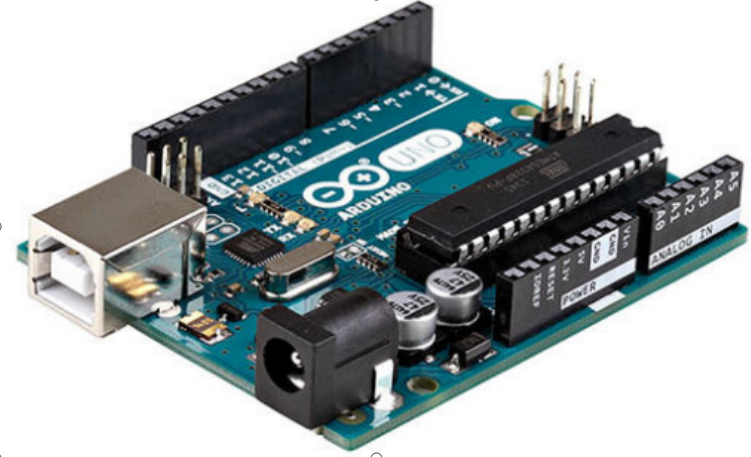
\includegraphics[width=2in]{Images/Intro_Arduino/arduino_uno.png}
    }
    \subfloat[Raspberry Pi 2 Model B]{
        \label{fig : raspberry_pi_2}
        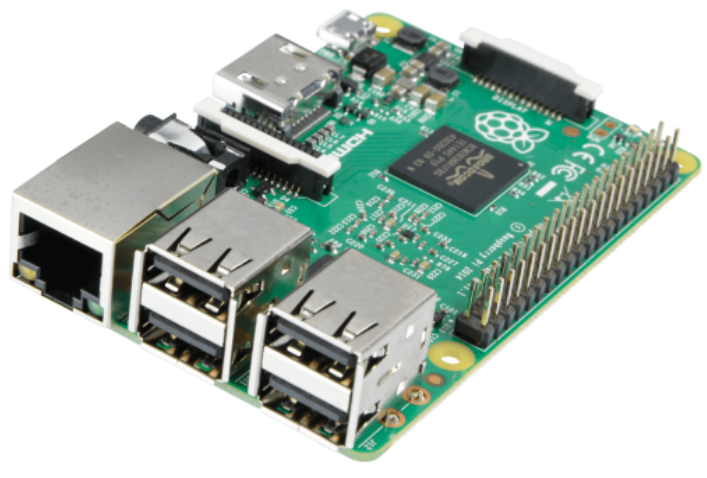
\includegraphics[width=2in]{Images/Intro_Arduino/raspberry.png}
    }
    \caption{Development boards}
\end{figure}

\section{Micro-controllers and Micro-processors}
Micro-controllers and Micro-processors are common terms used in \ac{IoT} and embedded systems. It is worth a while to understand the difference between them, to choose which is better to our project need.
\paragraph{ } Micro-controllers and micro-processors are used to execute instructions and control various units interfaced with them. However their complexity and utility can vary greatly. Micro controllers are similar to a small computer fabricated into a single \ac{IC}. It contains a processor core, ROM, RAM, and I/O pins It does not need any external circuits to do its task. It can manage memory and other services its own. It does the job of managing units as well an performing calculations. Micro-processor, on the other hand, has only CPU inside them. It does not have RAM, ROM of its own. Processors are dedicated to perform calculations. They depend on external circuits for its peripheral like RAM, ROM to work. They are used where the task are complex and tricky. The features are summarized in table \ref{tab:compare_micro_proc}.

\begin{figure}
    \centering
    \subfloat[Microprocessor]{
        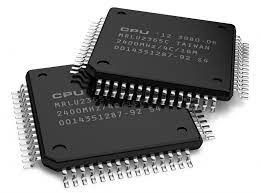
\includegraphics[width=1.2in]{Images/Intro_Arduino/processor.jpeg}
    }\qquad
    \subfloat[Micro-controller]{
        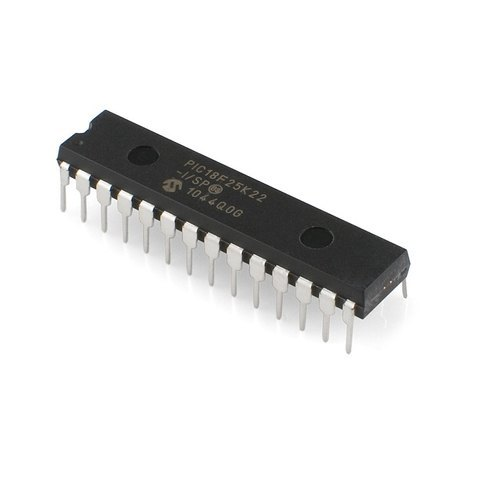
\includegraphics[width=1.2in]{Images/Intro_Arduino/microcontroller.jpg}
    }
    \caption{Processor and Micro-Controllers}
\end{figure}

\begin{table*}
    \renewcommand{\arraystretch}{1.5}
    \resizebox{5in}{!}{%
        \begin{tabular}{|l|l|}
        \hline
        \multicolumn{1}{|c|}{\textit{\textbf{Micro processor}}} &
          \multicolumn{1}{c|}{\textit{\textbf{Micro controller}}} \\ \hline
        RAM, ROM, EEPROM needs to be connected         & RAM, ROM, EEPROM are present on single IC \\ \hline
        Expensive                                      & Cheap                                     \\ \hline
        High processing speed (\textgreater{}1Ghz)     & Low processing speed (\textless{}50Mhz)   \\ \hline
        No power saving technology                     & Optimized power usage                     \\ \hline
        Used in large applications                     & Used in small application                 \\ \hline
        Process complex task                           & Process simple task                       \\ \hline
        Dissipate high heat. Might need cooling        & Does not dissipate high heats.            \\ \hline
        \begin{tabular}[c]{@{}l@{}}Usage of external storage\\ (HardDisk - GB of spaces)\end{tabular} &
          \begin{tabular}[c]{@{}l@{}}Usage of internal Storage\\ (EEPROM - few KB space)\end{tabular} \\ \hline
        Eg: Intel Pentium 4, Intel Core i7, AMD Athlon & Eg: ATmega328, ESP8266, ESP32, ATMEGA32U4 \\ \hline
        Board: Raspberry Pi                            & Board: Arduino                            \\ \hline
        \end{tabular}%
    }
    \vspace{0.5cm}
    \caption[Microprocessors VS Micro-controllers]{Comparison of Microprocessors and Micro-controllers}
    \label{tab:compare_micro_proc}
\end{table*}

\section{Arduino Boards}
Arduino is a large community that develops various micro-controller boards. Depending on the project application and usage, various customized official boards are available. The most generally used Arduino board is the “Arduino Uno”. We would be making use of Arduino Uno to develop various projects.

\begin{figure*}
  \centering
  \subfloat[Arduino Due]{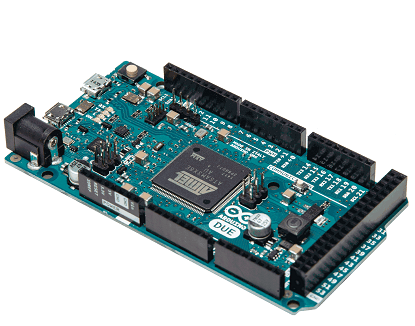
\includegraphics[width=2in]{Images/Intro_Arduino/ard_due.png}} \quad
  \subfloat[Arduino Leonardo]{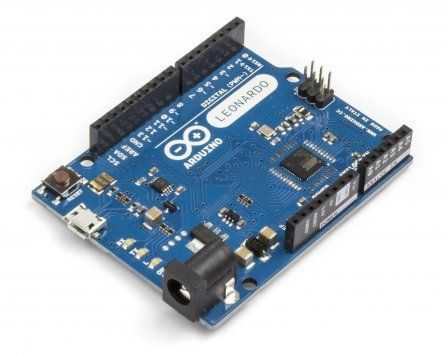
\includegraphics[width=2in]{Images/Intro_Arduino/ard_leonardo.jpg}}\quad
  \subfloat[Arduino Uno R3]{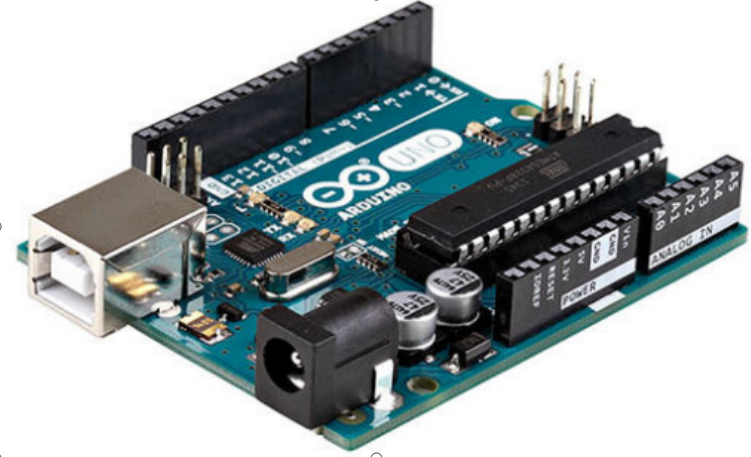
\includegraphics[width=2in]{Images/Intro_Arduino/arduino_uno.png}}\\
  \subfloat[Arduino Mega 2560]{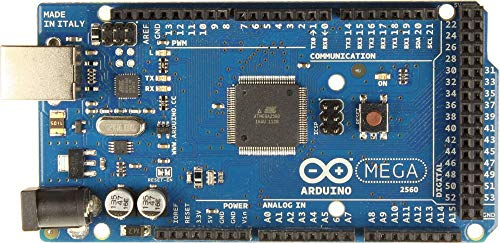
\includegraphics[width=2in]{Images/Intro_Arduino/ard_mega.jpg}}\quad
  \subfloat[Arduino Nano]{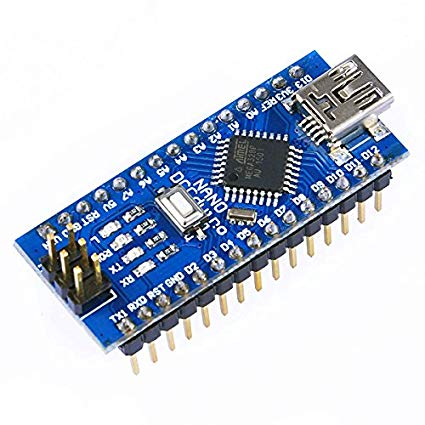
\includegraphics[width=2in]{Images/Intro_Arduino/ard_nano.jpg}}\quad
  \subfloat[LillyPad Arduino]{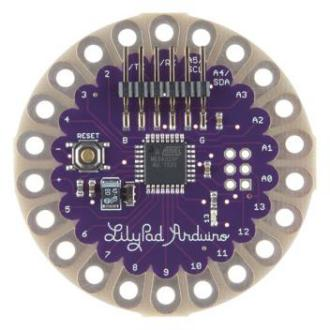
\includegraphics[width=2in]{Images/Intro_Arduino/ard_lillypad.jpg}}
  \caption{Arduino Boards}
\end{figure*}

\begin{figure}
    \centering
    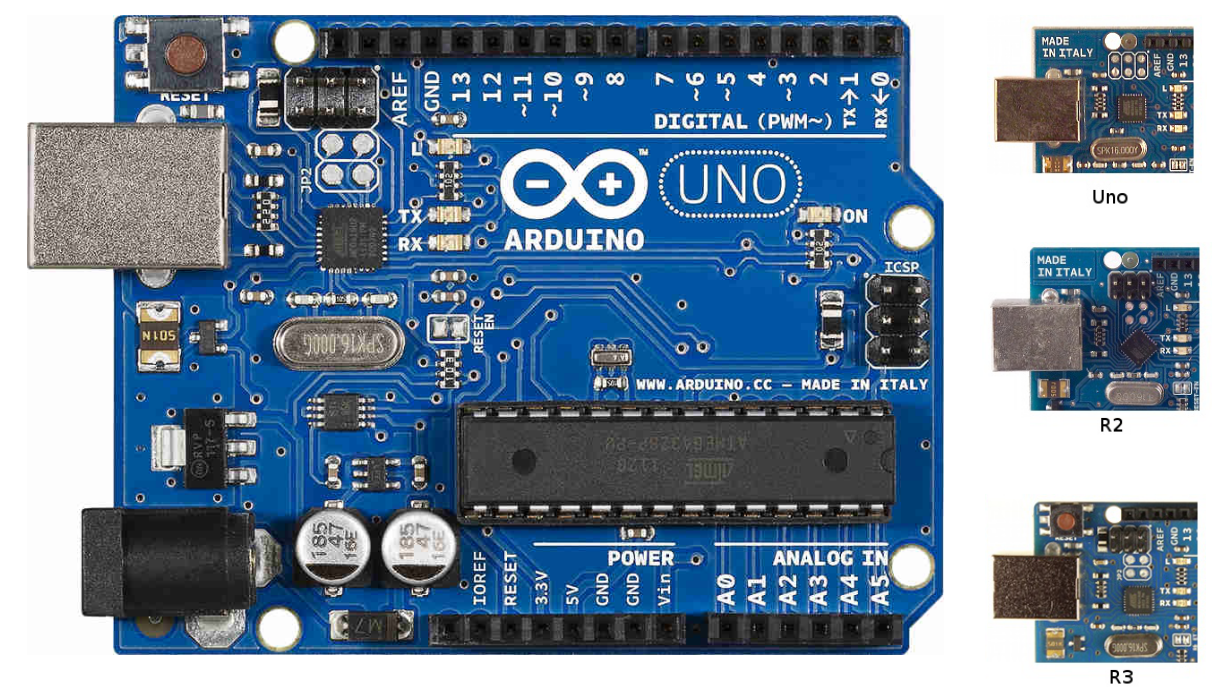
\includegraphics[width=4.3in]{Images/Intro_Arduino/arduino_uno_versions.png}
    \caption[Arduino Uno version]{Arduino Uno versions. Notice the alignment and position of ATMega16U2 micro-controller}
\end{figure}
\newpage

\section{Arduino Uno R3}
    \subsection{On-board units}
    
    \begin{figure}
        \centering
        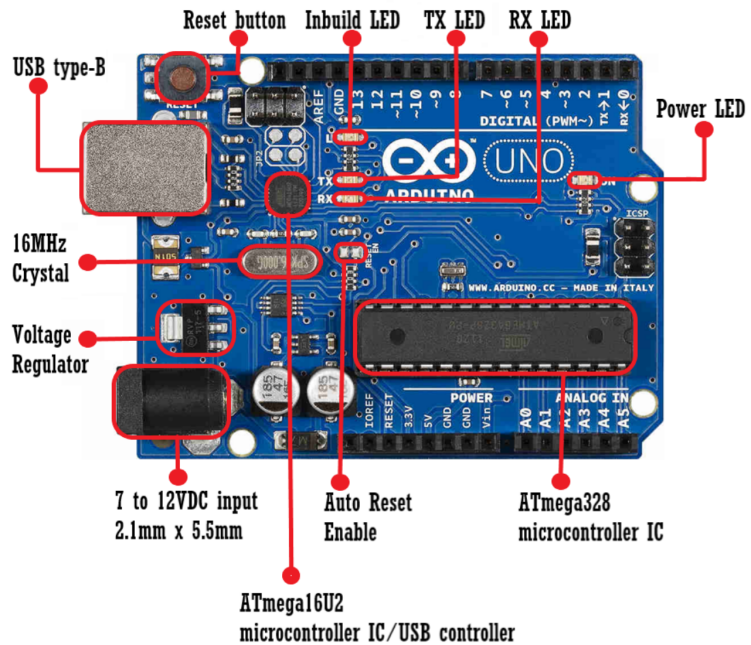
\includegraphics[width=\textwidth]{Images/Intro_Arduino/uno_desp.png}
        \caption{Arduino Uno R3 Pinout}
    \end{figure}
    
    \begin{itemize}
        \item ATmega328 micro controller \\
        Heart of Arduino Uno R3. This micro controller unit executes instructions. Programs are stored inside this unit.
        \item ATmega16U2 micro controller\\
        Used to assist main micro controller. Placed near to USB port to decode USB information. Stands as a boot loader that write programs into main micro controller. The transmit LED (Tx LED) and receive (Rx LED) turns on whenever read or write operations are performed to micro-controllers. 
        \item 16Mhz\\
        Act as heart beat of Arduino board. Serves as clock for timing various signals.
        \item Use type-B\\
        Used to interface Arduino to computer. Arduino board can be programmed via USB. Serial communication with board and serial monitor can also be achieved.
        \item 12V DC input\\
        The board can be powered via 12V DC adapter. The 12V is passed via capacitors to provide enough ampere and voltage across the board.
        \item Voltage regulator\\
        The digital circuits usually work at 5V. The 5V voltage regulator ensures that all the units gets proper voltage levels. If the board is successfully powered, the power LED glow brightly.
        \item Reset Button\\
        At time we might need to restart the board from the beginning. The reset button is used to reload the program from start. The reset can also be triggered inside the program.
    \end{itemize}
    
    \subsection{Micro controller : ATmega328}
    
    \begin{table}
        \centering
        \begin{tabular}{|l|l|}
            \hline
            \multicolumn{1}{|c|}{\textit{\textbf{Parameter}}} & \multicolumn{1}{c|}{\textit{\textbf{Value}}} \\ \hline
            CPU Type                    & 8-bit AVR       \\ \hline
            Performance                 & 20MIPS at 20MHz \\ \hline
            Flash Memory                & 32 KB           \\ \hline
            SRAM                        & 2 KB            \\ \hline
            EEPROM                      & 1 KB            \\ \hline
            Pin Count                   & 28 or 32 pins   \\ \hline
            Maximum operating frequency & 20Mhz           \\ \hline
            Maximum I/O pins            & 23              \\ \hline
            External Interrupts         & 2               \\ \hline
            Board: Raspberry Pi         & Board: Arduino  \\ \hline
        \end{tabular}
        \caption{ATmega328 spec}
    \end{table}

\section{Pin Layout}
Pins of Arduino can be broadly divided into two categories depending on their utility. For each pin, there is a marking on the board to denote the function of that pin. Pins are divided into:
\begin{enumerate}
    \item General Purpose Input Output pins ( total 20 pins )\\ 
    The functions of these pins can be programmed as per user need. They can either act as input pins or output pins. Input pins are those pins which Arduino would be listening for voltage variations. Output pins are those pins where Arduino controls the output voltage. These pins can also be classified into two categories. They are 
    \begin{itemize}
        \item Digital Pins
        \item Analog Pins
    \end{itemize}
    
    \item Special Purpose pins (total 9 pins)\\
    The functions of these pins are predetermined and cannot be changed. They are reserved for special purpose. They include VCC (5v and 3.3v) , Vin, GND, RESET, IOREF, AREF, ICSP header.
    
    \par VCC pins provide a fixed output voltage, acting as a positive terminal of a cell. GND pin provide a fixed zero voltage. They act as the negative terminal of a cell. Any additional components that need to be interfaced with Arduino would surely be connected to GND pin. Vin pin is used to power up the Arduino. Depending on how the board is powered, Vin pin can also act as 5v VCC pin.
    \par RESET pin have the function similar to RESET push button. They can cause the program to restart from the beginning. IOREF and AREF stands for Input-output reference and Analog reference pin. They stand as a reference point to calculate voltages at digital and Analog pins. \ac{ICSP} header pins are place close to micro-controllers. It is the ability of a micro-controller to be programmed without disconnecting from the circuitry.
\end{enumerate}

\section{Methods to power up Arduino}
There are mainly three ways to power up the board. 
\par The first method is to use UBS cable to power up the device. Just connect USB port to computer or a power bank. In this method the Vin pin can act as a 5V output pin. Make sure you don’t draw much power so as the damage the port. The 12V DC jack should be kept free. 
\par The second method is the power up via 12V DC jack. This will cause the board to have a bit higher current to handle components connect to it. The Vin pin act as a constant 5V DC output pin. In this method the USB port should to kept free. To make serial communication, make use of pins 0,1. 
\par The third pin is to power 5V via Vin pin. The 12V jack and USB must be kept free. In this method, the board is likely to run on lower ampere.

\section{Digital Pins}
\par Digital pins are those pins that act on digital values. A positive 5V (above 2.5V) act as binary 1 or HIGH digital signal. A ground 0V (below 2.3V) act as binary 0 or LOW digital signal. Arduino being a digital system, all general purpose input-output pins can be used as digital pins. There are total of 20 pins that can be used for digital signals, ranging from pin 0 to pin13 and A0 to A5. To make use of digital signals we make use of functions like digitalRead() and digitalWrite().

\begin{figure}
 \centering
 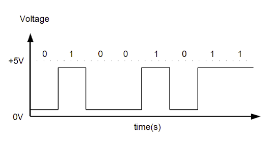
\includegraphics[width=3.5in]{Images/Intro_Arduino/digital_graph.png}
 \caption{Digital signals}
\end{figure}

\section{Analog Pins}
\par The pins that support analog input are called analog pins. Analog signals are those signals that vary continuously. That is, they do not have a specific cutoff like digital signals. They can assume wide range of values. Temperature is an example of analog signals that vary continuously. Since Arduino is an digital circuit, the analog signals needs to be converted to digital signals for the micro controller to understand. This function is performed by \ac{ADC}. \ac{ADC} convert analog signal to 10bit digital value by sampling the signal and then mapping each sample to $2^{10}$ levels. There are a total of 6 pins in Arduino Uno that supports \ac{ADC}, ranging from pins A0 to A5. To read analog value we make use of function analogRead().

\begin{figure}
 \centering
 \includegraphics[width=\textwidth]{Images/Intro_Arduino/analog_graph.png}
 \caption{Analog signals}
\end{figure}

\section{\ac{PWM}}
\ac{PWM} is the technique used to convert the digital signals to analog output results from Arduino. Arduino cannot directly produce various voltage levels. Being a digital circuit, it can only produce voltage levels 0V and 5V. To stimulate an analog effect, it creates square waves. The square wave have two key components: frequency and duty cycle. Frequency stays constant of about 500 Hz whereas the duty cycle is manipulated. Duty cycle refers to the amount of time signal stays high in a given time cycle. If Duty cycle is 100\%, we would get an effect of 100\% of 5V = 5V. If Duty cycle is 50\%, we would get an effect of 50\% of 5V = 2.5V. 

\par Arduino Uno can support \ac{PWM} on its 6 selected pins. They are pins 3, 5, 6, 9, 10 and 11. These pins have a tilde symbol ( \textasciitilde{} ) associated with their pin number on the board. The analog output function accepts 8 bit numbers, that are mapped to duty cycle. The 8 bit numbers can produce $2^8=256$ possible variations, spanning from zero to 255. The function analogWrite() is used to  produce analog output from Arduino at \ac{PWM} pins.

\begin{figure}
 \centering 
 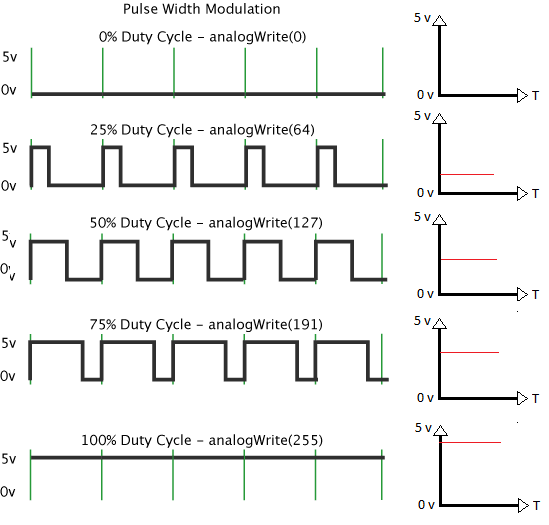
\includegraphics[width=3.5in]{Images/Intro_Arduino/pwm.png}
 \caption{Pulse width Modulation}
\end{figure}

\renewcommand{\arraystretch}{1.2}
\begin{table}
	\raggedright
    \resizebox{\textwidth}{!}{%
        \begin{tabular}{|l|l|}
        \hline
        \multicolumn{1}{|c|}{\textit{\textbf{ADC}}} & \multicolumn{1}{c|}{\textit{\textbf{PWM}}} \\ \hline
        Analog to Digital Converter                 & Pulse Width Modulation                     \\ \hline
        \begin{tabular}[c]{@{}l@{}}Implements sampling on analog \\ signals to convert to digital values\end{tabular} &
          \begin{tabular}[c]{@{}l@{}}Uses width of the pulse ( duty cycle) to \\ convert digital to analog signals\end{tabular} \\ \hline
        10 bit resolution : input                   & 8 bit resolution : output                  \\ \hline
        Applicable only on A0 to A5                 & Applicable only on 3, 5, 6, 9, 10, 11      \\ \hline
        analogRead()                                & analogWrite()                              \\ \hline
        \end{tabular}%
    }
    \caption{ADC v/s PWM}
\end{table}
\renewcommand{\arraystretch}{1}

\newpage
\begin{figure*}
    \centering
    \includegraphics[height=8.25in]{Images/Intro_Arduino/datasheet.png}
    \caption{Arduino Uno Data-sheet}
\end{figure*}









